% XeLaTeX, two passes. Standalone folder: images/ and data/ travel with main.tex.
\RequirePackage{fix-cm}
\documentclass[aspectratio=169,10pt]{beamer}
\usepackage{fontspec}
\setsansfont{Arial}
\setmainfont{Arial}
\usefonttheme{professionalfonts}
\usepackage{amsmath,booktabs,array,colortbl,graphicx,pgfplots}
\pgfplotsset{compat=1.18}
% Lecture-style theme: white canvas, gray title band and blue footer.
\definecolor{Navy}{HTML}{12366D}
\definecolor{Blue}{HTML}{1458B5}
\definecolor{MidBlue}{HTML}{4D84C6}
\definecolor{Teal}{HTML}{1458B5}
\definecolor{Orange}{HTML}{4D84C6}
\definecolor{Muted}{HTML}{5E6672}
\definecolor{Light}{HTML}{E8F0FA}
\definecolor{TitleBand}{HTML}{F2F2F2}
\setbeamercolor{normal text}{fg=black,bg=white}
\setbeamercolor{frametitle}{fg=Blue,bg=TitleBand}
\setbeamercolor{structure}{fg=Blue}
\setbeamercolor{alerted text}{fg=Blue}
\setbeamercolor{foot author}{fg=white,bg=Blue}
\setbeamercolor{foot course}{fg=Blue,bg=TitleBand}
\setbeamercolor{foot title}{fg=Navy,bg=Light}
\setbeamercolor{foot page}{fg=Blue,bg=TitleBand}
\setbeamerfont{frametitle}{size=\fontsize{14}{17}\selectfont,series=\mdseries}
\setbeamerfont{footline}{size=\fontsize{7}{8.5}\selectfont}
\setbeamertemplate{navigation symbols}{}
\setbeamertemplate{itemize item}[ball]
\setbeamertemplate{itemize subitem}[circle]
\setbeamersize{text margin left=8mm,text margin right=8mm}
\setbeamertemplate{frametitle}{%
  \nointerlineskip
  \begin{beamercolorbox}[wd=\paperwidth,sep=0pt,leftskip=4mm,rightskip=4mm]{frametitle}
    \vbox{}\vskip0.6mm
    \usebeamerfont{frametitle}\strut\insertframetitle\strut\par
    \vskip0.6mm
  \end{beamercolorbox}%
}
\newcommand{\insertpaperreference}{}
\newcommand{\paperreference}[1]{\gdef\insertpaperreference{#1}}
\setbeamertemplate{footline}{%
  \leavevmode\hbox{%
    \begin{beamercolorbox}[wd=.12\paperwidth,ht=2.3mm,dp=0.6mm,center]{foot author}%
      \usebeamerfont{footline}Nhóm 2
    \end{beamercolorbox}%
    \begin{beamercolorbox}[wd=.16\paperwidth,ht=2.3mm,dp=0.6mm,center]{foot course}%
      \usebeamerfont{footline}Xử lý ảnh
    \end{beamercolorbox}%
    \begin{beamercolorbox}[wd=.60\paperwidth,ht=2.3mm,dp=0.6mm,center]{foot title}%
      \usebeamerfont{footline}\fontsize{6.5}{7.5}\selectfont\insertpaperreference
    \end{beamercolorbox}%
    \begin{beamercolorbox}[wd=.12\paperwidth,ht=2.3mm,dp=0.6mm,center]{foot page}%
      \usebeamerfont{footline}\insertframenumber\ /\ \inserttotalframenumber
    \end{beamercolorbox}%
  }%
}
\setbeameroption{hide notes}
\setlength{\parskip}{4pt}
\graphicspath{{images/}}
\newcommand{\captionnote}[1]{\par\vspace{1mm}{\fontsize{7}{8.5}\selectfont\color{Muted}#1\par}}
\newcommand{\takeaway}[1]{\par\vspace{2mm}{\color{Teal}\bfseries#1\par}}
\newcommand{\smalltable}{\fontsize{9}{11}\selectfont\renewcommand{\arraystretch}{1.25}}
\pgfplotsset{slideplot/.style={
  width=10.5cm,height=5.25cm,
  axis lines=left,axis line style={Muted!50},
  tick label style={font=\scriptsize,color=Muted},
  label style={font=\small},
  legend style={font=\scriptsize,draw=none,fill=none},
  ymajorgrids=true,grid style={Light},
  tick align=outside,clip=false,
  every axis plot/.append style={line width=1.2pt,mark size=2pt}
}}
\hypersetup{pdftitle={Xử lý ảnh thiếu sáng cho nhận dạng biển báo giao thông},pdfauthor={Nhóm 2, Đại học Phenikaa}}
\begin{document}

% 01
\paperreference{}
\begin{frame}{Bài tập lớn môn Xử lý ảnh}
\begingroup\setlength{\parskip}{2pt}
\begin{columns}[T,onlytextwidth]
\column{0.83\textwidth}
{\small ĐẠI HỌC PHENIKAA\par TRƯỜNG CÔNG NGHỆ THÔNG TIN PHENIKAA}
\column{0.12\textwidth}

\includegraphics[width=1.2cm]{phenikaa.jpg}
\end{columns}
\par\vspace{4mm}
{\fontsize{18}{22}\selectfont\bfseries
Khảo sát ảnh hưởng của xử lý ảnh\par
đến hiệu năng nhận dạng biển báo\par
giao thông trong điều kiện thiếu sáng\par}
\par\vspace{2mm}
{\small\textbf{Giảng viên hướng dẫn:} TS. Nguyễn Ngọc Giang\par}
{\fontsize{8}{10}\selectfont\textbf{Nhóm 2}\par
\begin{tabular}{@{}lll@{}}
Kiều Thị Thu Trang & 24100093 & 24100093@st.phenikaa-uni.edu.vn\\
Trần Minh Sang & 24100012 & 24100012@st.phenikaa-uni.edu.vn\\
Ngô Quang Thiện & 24102651 & 24102651@st.phenikaa-uni.edu.vn
\end{tabular}\par}
{\scriptsize GTSRB \qquad ResNet-18 \qquad Tháng 10/2026}
\endgroup
\note{Thời lượng khoảng 30 giây. Giới thiệu tên đề tài và thành viên. Nhấn mạnh đối tượng khảo sát là các phép xử lý ảnh, còn ResNet-18 đóng vai trò bộ nhận dạng cố định để kiểm chứng. Logo và thông tin nhóm lấy từ paper mẫu theo yêu cầu người dùng.}
\end{frame}

% 02
\paperreference{}
\begin{frame}{1.1. Mục tiêu và phạm vi}\relax
{\fontsize{19}{24}\selectfont\bfseries Ảnh sáng hơn có giúp\par nhận dạng biển báo chính xác hơn?\par}
\par\vspace{5mm}
\begin{columns}[T,onlytextwidth]
\column{0.47\textwidth}
\textbf{Khảo sát xử lý ảnh}\par
Mô phỏng tối và nhiễu ở 3 mức.\par
So sánh 7 enhancer, 3 bộ lọc và hai thứ tự.\par
Đo PSNR, SSIM và hiệu năng nhận dạng.
\column{0.47\textwidth}
\textbf{Phạm vi thực nghiệm}\par
Đầu vào là crop biển báo GTSRB.\par
ResNet-18 phân loại 43 lớp.\par
Chưa khảo sát detector hoặc camera đêm thực.
\end{columns}
\takeaway{Chọn tiền xử lý theo mục tiêu nhận dạng trên validation.}
\note{Khoảng 45 giây. Ảnh tăng sáng có thể dễ nhìn hơn nhưng cũng có thể khuếch đại nhiễu hoặc làm sai nét số. Đề bài cần đánh giá cả chất lượng ảnh và tác vụ nhận dạng. Dùng crop đã có ROI, không tuyên bố hệ thống phát hiện biển báo toàn cảnh. Nguồn: đề bài người dùng, README.md và báo cáo mục 1.}
\end{frame}

% 03
\paperreference{\href{https://doi.org/10.1109/IJCNN.2011.6033395}{Stallkamp et al., IJCNN 2011}}
\begin{frame}{1.2. GTSRB và chuẩn hóa đầu vào}\relax
\begin{columns}[T,onlytextwidth]
\column{0.49\textwidth}
{\fontsize{30}{33}\selectfont\bfseries 43}\par
lớp biển báo giao thông\par\vspace{3mm}
\smalltable
\begin{tabular}{lr}
\rowcolor{Blue} \color{white}\bfseries Tập dữ liệu & \color{white}\bfseries Số ảnh\\\midrule
Train & 31.350\\
Validation & 7.829\\
Cách ly & 30\\
Official test & 12.630\\\bottomrule
\end{tabular}
\column{0.47\textwidth}
\textbf{Chuẩn hóa ảnh}\par
Cắt ROI, thêm lề 5\%.\par
RGB $64\times64$, cường độ $[0,1]$.\par
Chia train/validation theo track để hạn chế rò rỉ dữ liệu.\par\vspace{3mm}
\textbf{Tập con khảo sát}\par
1.290 ảnh validation chọn tham số.\par
430 ảnh test, 10 ảnh mỗi lớp.
\end{columns}
\note{Khoảng 45 giây. Giải thích track là chuỗi ảnh liên tiếp của cùng một biển. Chia ở cấp track tránh các ảnh gần giống nhau nằm ở cả train và validation. 30 ảnh cách ly không thuộc tập train cuối. Subset cân bằng có 430 ảnh; full-test 12.630 ảnh đã được kiểm tra dự đoán thô. Nguồn: configs/resnet18.json; src/data.py; report/evidence/final/audit.json.}
\end{frame}

% 04
\paperreference{}
\begin{frame}{2.1. Mô phỏng thiếu sáng và nhiễu}\relax
\par\vspace{-1mm}
\[U=X^{\gamma_d},\qquad V=\mathcal{P}(pU)/p,\qquad
Y=\operatorname{clip}(V+\varepsilon,0,1)\]
\par\vspace{-3mm}
\begin{columns}[c,onlytextwidth]
\column{0.68\textwidth}
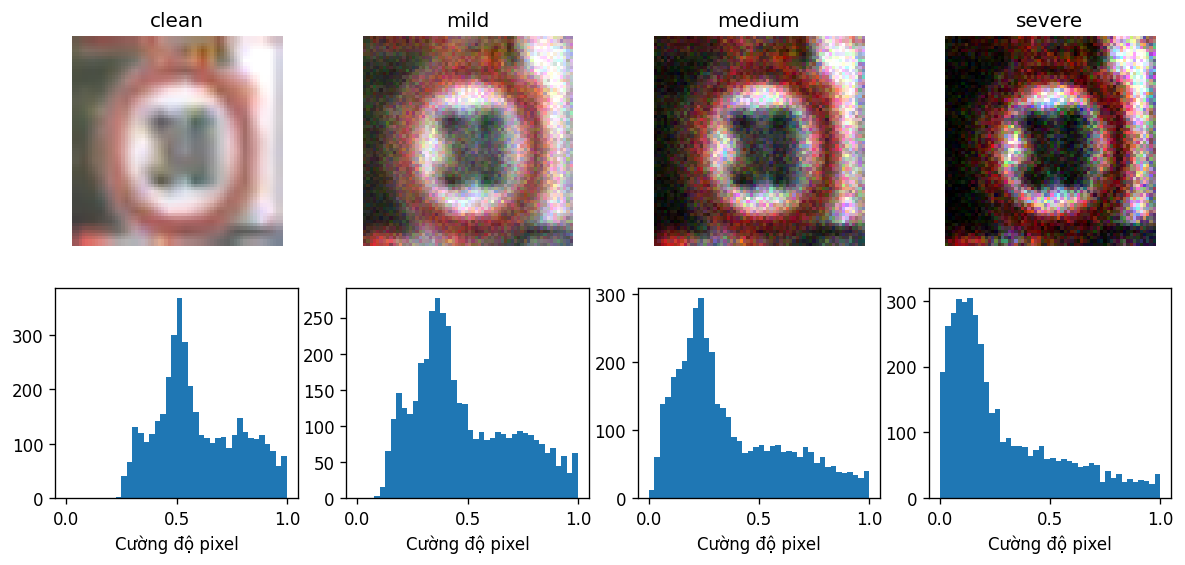
\includegraphics[width=\linewidth]{degradation.png}
\column{0.29\textwidth}
\setlength{\tabcolsep}{3pt}\smalltable
\begin{tabular}{lrrr}
\rowcolor{Blue} \color{white}\bfseries  & \color{white}\bfseries $\gamma_d$ & \color{white}\bfseries $p$ & \color{white}\bfseries $\sigma_n$\\\midrule
Nhẹ & 1,5 & 120 & 0,005\\
Vừa & 2,2 & 60 & 0,010\\
Nặng & 3,0 & 30 & 0,020\\\bottomrule
\end{tabular}
\par\vspace{2mm}\par
{\small $\varepsilon\sim\mathcal{N}(0,\sigma_n^2)$\par
Gamma làm tối.\par
Poisson phụ thuộc tín hiệu.\par
Gaussian là nhiễu cộng.}
\end{columns}
\captionnote{Minh họa cùng một crop validation, noise seed 101.}
\note{Khoảng 60 giây. Đọc thứ tự: Gamma rồi Poisson, Gaussian, cuối cùng clip. Chỉ vào histogram dịch về phía tối và vùng chữ số bị nhiễu. Giải thích p càng nhỏ thì nhiễu Poisson càng mạnh tương đối. Đây là mô phỏng trên RGB, không phải mô hình vật lý đầy đủ của cảm biến. Nguồn: src/degradation.py, configs/resnet18.json; hình lấy nguyên từ notebook cell 7.}
\end{frame}

% 05
\paperreference{\href{https://doi.org/10.1109/CVPR42600.2020.00185}{Guo et al., CVPR 2020}; \href{https://doi.org/10.1109/ICCV51070.2023.01149}{Cai et al., ICCV 2023}; \href{https://doi.org/10.1145/3618373}{Jiang et al., ACM TOG 2023}}
\begin{frame}{3.1. Bảy phương pháp tăng cường ảnh}\relax
\centering
\smalltable
\begin{tabular}{p{3.3cm}p{9.4cm}}
\rowcolor{Blue} \color{white}\bfseries Phương pháp & \color{white}\bfseries Cơ chế chính\\\midrule
Gamma & Điều chỉnh cường độ bằng hàm lũy thừa\\
HE & Cân bằng histogram toàn cục trên kênh Y\\
CLAHE & Cân bằng cục bộ và giới hạn tương phản\\
MSR (Retinex) & Chênh lệch log với ảnh làm mờ ở nhiều tỉ lệ\\
Zero-DCE & Học đường cong tăng sáng theo ảnh\\
Retinexformer & Phục hồi bằng thông tin chiếu sáng và Transformer\\
Diffusion & Phục hồi có điều kiện trong miền wavelet\\\bottomrule
\end{tabular}
\par\vspace{3mm}\par
\raggedright
\textbf{Identity:} giữ ảnh tối làm đối chứng. \quad
\textbf{Clean:} ảnh gốc tham chiếu.
\captionnote{Ba bộ tăng cường sâu dùng trọng số tác giả, không huấn luyện lại trên GTSRB.}
\note{Khoảng 45 giây. Phân biệt bốn phương pháp truyền thống và ba phương pháp học sâu. Tổng cộng tám nhánh đánh giá khi tính Identity. Không coi Clean là một thuật toán tăng cường. Nguồn: src/enhancement.py. Zero-DCE: https://arxiv.org/abs/2001.06826; Retinexformer: https://arxiv.org/abs/2303.06705; diffusion: https://arxiv.org/abs/2306.00306.}
\end{frame}

% 06
\paperreference{}
\begin{frame}{3.2. Gamma và lựa chọn mức tăng sáng}\relax
\begin{columns}[c,onlytextwidth]
\column{0.43\textwidth}
{\large $\widehat{X}=Y^{\alpha},\quad 0<\alpha<1$}\par\vspace{3mm}
$\alpha$ nhỏ nâng sáng mạnh hơn.\par
Vùng tối cũng dễ khuếch đại nhiễu.\par\vspace{3mm}
\textbf{Lưới khảo sát}\par
$\alpha\in\{0,4;\ 0,6;\ 0,8\}$\par
Validation chọn \alert{$\alpha=0,8$}.
\column{0.54\textwidth}
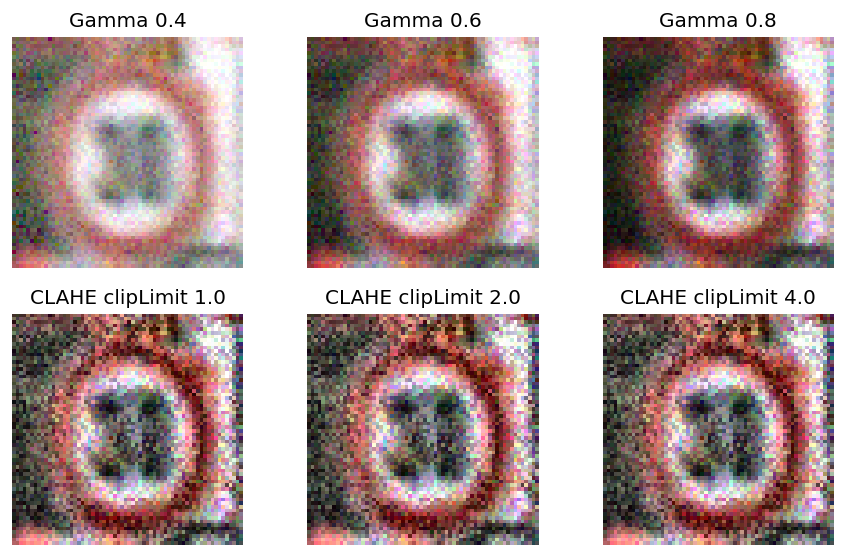
\includegraphics[width=\linewidth]{parameters.png}
{\scriptsize\color{Muted}Hàng trên: Gamma. Hàng dưới: CLAHE với lưới $8\times8$.}
\end{columns}
\takeaway{Tham số tăng sáng cần chọn bằng validation.}
\note{Khoảng 50 giây. Chỉ vào ba ảnh trên để so mức nâng sáng. Ở vùng tối đạo hàm alpha nhân Y mũ alpha trừ 1 có thể lớn, vì thế nhiễu được khuếch đại. Hàng dưới dùng để minh họa CLAHE; giữ lưới 8x8 nên đây không phải cấu hình được chọn cuối. Nguồn: notebook cell 9 và cell 13; src/enhancement.py.}
\end{frame}

\paperreference{}
\begin{frame}{3.3. HE: ánh xạ từ phân phối tích lũy}\relax
\begin{columns}[T,onlytextwidth]
\column{0.48\textwidth}
\textbf{Từ histogram đến mức sáng mới}
\[p(k)=n_k/N,\qquad C(k)=\sum_{j=0}^{k}p(j)\]
\[T(k)=\operatorname{round}\!\left(255\frac{C(k)-C_{\min}}{1-C_{\min}}\right)\]
{\small $n_k$: số pixel ở mức $k$; $N$: tổng pixel.\par
$C_{\min}$: CDF khác 0 đầu tiên.}
\column{0.48\textwidth}
\textbf{Cài đặt trong dự án}\par
RGB $\rightarrow$ YCrCb $\rightarrow$ HE trên Y.\par
Giữ Cr, Cb rồi chuyển về RGB.\par
Lượng tử hóa 8 bit trước xử lý.
\par\vspace{3mm}
\textbf{Điểm mạnh và giới hạn}\par
Nhanh, không chọn tham số tăng sáng.\par
Một ánh xạ chung cho toàn ảnh; vùng nhiễu cũng bị kéo giãn.
\end{columns}
\takeaway{Histogram trải rộng hơn chưa chứng minh nét biển báo rõ hơn.}
\captionnote{Ảnh hằng được xử lý riêng.}
\note{Khoảng 50 giây. Giải thích CDF là phần pixel có mức sáng không vượt quá k. Mức sáng mới phụ thuộc vị trí tích lũy trong histogram. HE xử lý cả vùng biển và nền bằng một ánh xạ nên không thích ứng với chiếu sáng từng vùng. Chỉ xử lý kênh Y giúp hạn chế biến đổi màu, nhưng lượng tử hóa và clipping vẫn có thể làm thay đổi màu.}
\end{frame}

\paperreference{}
\begin{frame}{3.4. CLAHE: giới hạn tương phản theo từng vùng}\relax
\begin{enumerate}
\item Chia kênh Y thành các ô và tính histogram từng ô.
\item Cắt các bin vượt ngưỡng, phân phối lại phần dư.
\item Tạo ánh xạ CDF cục bộ và nội suy giữa các ô.
\end{enumerate}
\par\vspace{3mm}
\begin{columns}[T,onlytextwidth]
\column{0.48\textwidth}
\textbf{Clip limit}\par
Khảo sát $\{1,2,4\}$; chọn \alert{1}.\par
Giới hạn histogram, không phải ngưỡng độ sáng của pixel.
\column{0.48\textwidth}
\textbf{Lưới trên ảnh $64\times64$}\par
$4\times4$: mỗi ô khoảng $16\times16$ pixel.\par
$8\times8$: mỗi ô khoảng $8\times8$ pixel.\par
Validation chọn \alert{$4\times4$}.
\end{columns}
\takeaway{Ô quá nhỏ làm thống kê histogram nhạy hơn với nhiễu.}
\note{Khoảng 55 giây. Giải thích nội suy để tránh các khối vuông có ranh giới rõ. Clip limit hạn chế khuếch đại tương phản nhưng không thay thế bộ khử nhiễu. tileGridSize là số ô theo hai chiều, không phải kích thước pixel. Cấu hình được lựa chọn theo nhận dạng trên validation. Hình ở slide tiếp theo dùng cấu hình mặc định để minh họa cơ chế.}
\end{frame}

% 07
\paperreference{}
\begin{frame}{3.5. HE và CLAHE trên kênh độ sáng}\relax
\begin{columns}[T,onlytextwidth]
\column{0.48\textwidth}
\textbf{HE}\par
Một phép ánh xạ histogram cho toàn ảnh.
\column{0.48\textwidth}
\textbf{CLAHE}\par
Xử lý theo ô, giới hạn khuếch đại tương phản.
\end{columns}
\par\vspace{2mm}
\centering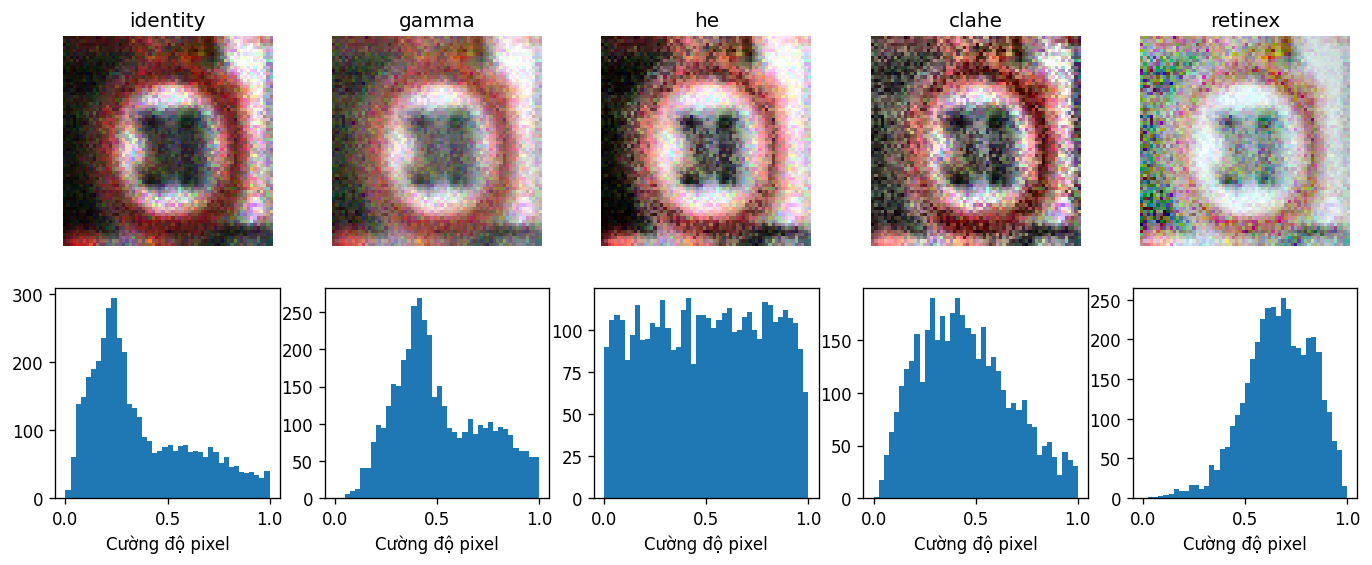
\includegraphics[width=12.5cm,height=3.5cm,keepaspectratio]{classical_default.png}\par
\raggedright
{\small RGB đổi sang YCrCb, xử lý Y rồi chuyển lại RGB.\par
Validation chọn CLAHE: \alert{clip limit 1, lưới $4\times4$}.}
\captionnote{Hình minh họa dùng tham số mặc định, riêng CLAHE là lưới $8\times8$.}
\note{Khoảng 60 giây. Histogram rộng hơn chưa chứng minh ảnh tốt hơn. HE có thể kéo giãn vùng sáng mạnh. CLAHE thích ứng theo vùng nhưng ô quá nhỏ trên ảnh 64x64 làm thống kê nhạy hơn với nhiễu. tileGridSize là số ô, không phải kích thước pixel của ô. Cấu hình chọn 4x4 tương ứng ô khoảng 16x16 pixel. Nguồn: src/enhancement.py; https://docs.opencv.org/4.x/d5/daf/tutorial_py_histogram_equalization.html.}
\end{frame}

% 08
\paperreference{\href{https://ntrs.nasa.gov/api/citations/19990005051/downloads/19990005051.pdf}{Jobson et al., IEEE TIP 1997}}
\begin{frame}{3.6. Retinex đa tỉ lệ và tính nhạy nhiễu}\relax
\textbf{Mô hình chiếu sáng và phản xạ:} $I=R\cdot L$
\par\vspace{2mm}
\[r=\frac{1}{S}\sum_{s=1}^{S}\left[\log(Y+\epsilon)-\log(G_{\sigma_s}*Y+\epsilon)\right]\]
\par\vspace{1mm}
\begin{columns}[T,onlytextwidth]
\column{0.48\textwidth}
\textbf{Cài đặt trong dự án}\par
Làm mờ Gaussian ở nhiều tỉ lệ.\par
Chuẩn hóa percentile 1--99\%.\par
Validation chọn $\sigma=[5,15,30]$.
\column{0.48\textwidth}
\textbf{Điểm cần kiểm chứng}\par
Log nhạy với dao động ở vùng tối.\par
Chi tiết và nhiễu đều có thể nổi rõ.\par
Không có bước khử nhiễu riêng.
\end{columns}
\takeaway{Ablation sẽ tách tác động của độ tối và từng loại nhiễu.}
\captionnote{MSR giản lược, không phải MSRCR có phục hồi màu riêng.}
\note{Khoảng 50 giây. Giải thích ảnh làm mờ là ước lượng chiếu sáng chậm biến thiên. Trừ trong miền log giúp làm rõ phản xạ nhưng không phân biệt biên thật với nhiễu. Tránh kết luận MSR luôn kém; thí nghiệm chỉ Gamma cho kết quả rất tốt và sẽ được trình bày ở phần ablation. Nguồn: src/enhancement.py và notebook cell 13.}
\end{frame}

\paperreference{\href{https://ntrs.nasa.gov/api/citations/19990005051/downloads/19990005051.pdf}{Jobson et al., IEEE TIP 1997}}
\begin{frame}{3.7. MSR: từ phản xạ ước lượng đến ảnh đầu ra}\relax
\textbf{Ba bước xử lý}\par
Làm mờ ở $\sigma=5,15,30$ $\rightarrow$ trừ log $\rightarrow$ lấy trung bình.
\par\vspace{3mm}
\textbf{Chuẩn hóa theo percentile}
\[\widehat{X}=\operatorname{clip}\!\left(\frac{r-q_1}{q_{99}-q_1},0,1\right)\]
{\small $q_1,q_{99}$ là percentile 1\% và 99\% trên mảng kết quả.}
\begin{columns}[T,onlytextwidth]
\column{0.48\textwidth}
\textbf{Tác dụng}\par
Giảm ảnh hưởng chiếu sáng chậm biến thiên.\par
Kết hợp chi tiết ở nhiều tỉ lệ.
\column{0.48\textwidth}
\textbf{Nguồn gây sai lệch}\par
Log và kéo giãn có thể tăng nhiễu.\par
Clipping làm mất giá trị ở hai đầu; màu có thể thay đổi.
\end{columns}
\captionnote{Nếu khoảng percentile quá nhỏ, trả lại ảnh đầu vào.}
\note{Khoảng 50 giây. Đây là MSR giản lược, không có phục hồi màu MSRCR. Nhiều tỉ lệ làm mờ không đồng nghĩa với có khử nhiễu riêng. Cần phân biệt khả năng xử lý ảnh chỉ tối với ảnh tối kèm nhiễu; thí nghiệm ablation phía sau cho thấy khác biệt rất lớn.}
\end{frame}

\paperreference{\href{https://doi.org/10.1109/CVPR42600.2020.00185}{Guo et al., CVPR 2020}}
\begin{frame}{3.8. Zero-DCE: học đường cong tăng sáng}\relax
\textbf{Đường cong điều chỉnh cường độ}
\[I_{t+1}=I_t+A_t\odot I_t\odot(1-I_t)\]
{\small $A_t$ được mạng ước lượng theo ảnh; $\odot$ là nhân từng phần tử.}
\par\vspace{3mm}
\begin{columns}[T,onlytextwidth]
\column{0.48\textwidth}
\textbf{Nguyên lý}\par
Điều chỉnh thích ứng theo vị trí.\par
Lặp đường cong để tăng khả năng biểu diễn.\par
Nghiên cứu gốc học với ràng buộc không cần ảnh tham chiếu ghép cặp.
\column{0.48\textwidth}
\textbf{Trong dự án}\par
Checkpoint Epoch99.pth của tác giả.\par
Chỉ suy luận, không học lại trên GTSRB.\par
Đưa ảnh đầu ra về miền $[0,1]$.
\end{columns}
\takeaway{Tăng sáng thích ứng vẫn cần kiểm tra nhiễu và độ rõ nét số.}
\note{Khoảng 50 giây. Công thức là quy ước dấu trong mô tả phương pháp gốc; tham số có thể làm tăng hoặc giảm cường độ. Mạng dự đoán cách điều chỉnh ảnh chứ không dùng một gamma cố định. Không cần cặp ảnh khi huấn luyện gốc không có nghĩa dự án đã huấn luyện mạng. Trong thí nghiệm chỉ nạp checkpoint.}
\end{frame}

\paperreference{\href{https://doi.org/10.1109/ICCV51070.2023.01149}{Cai et al., ICCV 2023}}
\begin{frame}{3.9. Retinexformer: phục hồi có hướng dẫn chiếu sáng}\relax
\begin{center}
\fcolorbox{Teal}{Light}{\strut Ảnh tối}\quad$\rightarrow$\quad
\fcolorbox{Teal}{Light}{\strut Ước lượng chiếu sáng}\par\vspace{3mm}
$\downarrow$\par\vspace{2mm}
\fcolorbox{Teal}{Light}{\strut Phục hồi bằng Transformer}\quad$\rightarrow$\quad
\fcolorbox{Teal}{Light}{\strut Ảnh tăng cường}
\end{center}
\par\vspace{3mm}
\begin{columns}[T,onlytextwidth]
\column{0.48\textwidth}
\textbf{Khác với MSR}\par
Học biểu diễn và quan hệ giữa các vùng.\par
Dùng thông tin chiếu sáng để hỗ trợ phục hồi suy giảm.
\column{0.48\textwidth}
\textbf{Cấu hình sử dụng}\par
Trọng số LOL-v1 của tác giả.\par
Kích thước cần chia hết cho 4.\par
Crop $64\times64$ đáp ứng trực tiếp.
\end{columns}
\captionnote{Sơ đồ nguyên lý giản lược.}
\note{Khoảng 50 giây. Sơ đồ diễn tả ý tưởng, không phải toàn bộ các lớp mạng. Retinexformer không phải phép MSR rồi thêm Transformer; nó học cách dùng thông tin chiếu sáng để phục hồi. Trọng số học trên miền khác GTSRB nên cần đo thực nghiệm, không mặc định tốt hơn CLAHE.}
\end{frame}

\paperreference{\href{https://doi.org/10.1145/3618373}{Jiang et al., ACM TOG 2023}}
\begin{frame}{3.10. Diffusion trong miền wavelet}\relax
\textbf{Ý tưởng phục hồi có điều kiện}\par
Wavelet tách thông tin tần số thấp và chi tiết tần số cao.\par
Diffusion phục hồi có điều kiện kết hợp xử lý thành phần tần số cao.
\par\vspace{3mm}
\begin{columns}[T,onlytextwidth]
\column{0.48\textwidth}
\textbf{Cấu hình trong dự án}\par
10 bước lấy mẫu; trọng số EMA.\par
Hạt giống suy luận theo mã ảnh.\par
Đệm đến bội số 32 nếu cần.
\column{0.48\textwidth}
\textbf{Kiểm soát đầu ra}\par
Lấy pred\_x, cắt về kích thước gốc.\par
Chặn giá trị trong $[0,1]$.\par
Giữ cấu hình đã chọn trên validation.
\end{columns}
\takeaway{Nhiều bước phục hồi làm tăng chi phí xử lý mỗi ảnh.}
\note{Khoảng 55 giây. Phân biệt diffusion phục hồi ảnh có điều kiện với sinh ảnh tự do. Wavelet giúp biểu diễn riêng phần biến thiên chậm và chi tiết; không có nghĩa tự động giữ đúng mọi nét số. EMA là trọng số trung bình trượt của mô hình. Sau phần minh họa sẽ so chất lượng ảnh, F1 và thời gian xử lý để đánh giá đánh đổi.}
\end{frame}

% 09
\paperreference{\href{https://doi.org/10.1109/CVPR42600.2020.00185}{Guo et al., CVPR 2020}; \href{https://doi.org/10.1109/ICCV51070.2023.01149}{Cai et al., ICCV 2023}; \href{https://doi.org/10.1145/3618373}{Jiang et al., ACM TOG 2023}}
\begin{frame}{3.11. Tăng cường học sâu trên cùng một ảnh}\relax
\begin{columns}[c,onlytextwidth]
\column{0.43\textwidth}
\centering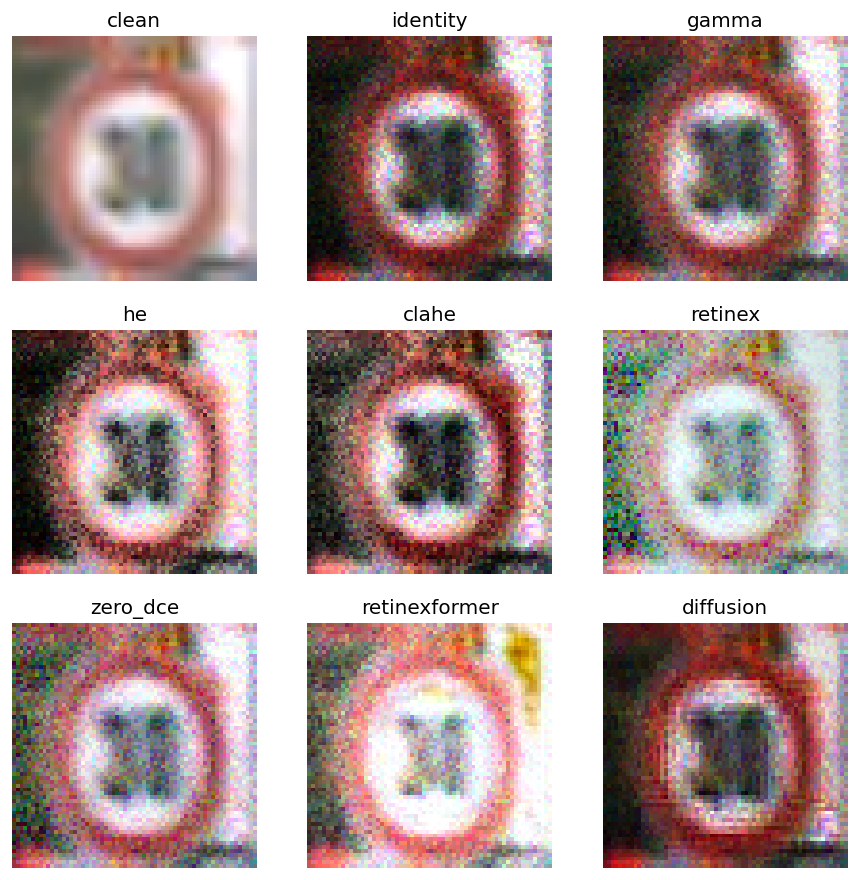
\includegraphics[height=5.7cm]{enhancers_selected.png}
\column{0.53\textwidth}
\textbf{Zero-DCE}\par
Ước lượng đường cong điều chỉnh pixel.\par\vspace{2mm}
\textbf{Retinexformer}\par
Phục hồi với biểu diễn chiếu sáng.\par\vspace{2mm}
\textbf{Wavelet-based diffusion}\par
10 bước lấy mẫu, dùng trọng số EMA.\par\vspace{3mm}
\alert{Độ sáng và màu đầu ra khác nhau rõ rệt.}\par
Cần đo thêm chất lượng và nhận dạng.
\end{columns}
\captionnote{Một crop validation mức vừa, tham số đã chọn.}
\note{Khoảng 50 giây. Hình này dùng tham số đã chọn, khác hình tham số mặc định ở phần HE và CLAHE. Nhìn vào nền trắng, viền đỏ và chữ số. Ảnh diffusion không sáng nhất nhưng giữ kết quả nhận dạng tốt trên tập khảo sát. Một mẫu chỉ minh họa cơ chế, không đại diện xếp hạng toàn tập. Nguồn và bài báo: notebook cell 14; https://arxiv.org/abs/2001.06826; https://arxiv.org/abs/2303.06705; https://arxiv.org/abs/2306.00306.}
\end{frame}

% 10
\paperreference{\href{https://doi.org/10.1109/CVPR.2016.90}{He et al., CVPR 2016}; \href{https://doi.org/10.1109/TIP.2003.819861}{Wang et al., IEEE TIP 2004}}
\begin{frame}{4.1. Giao thức đánh giá với ResNet-18 cố định}\relax
\begin{columns}[T,onlytextwidth]
\column{0.49\textwidth}
\textbf{Kiểm soát thí nghiệm}\par
Train clean với 3 seed: 11, 22, 33.\par
Giữ checkpoint cho mọi enhancer.\par
3 noise seed: 101, 202, 303.\par
Cùng ảnh tối cho mọi phương pháp.\par\vspace{3mm}
\textbf{219 lượt trên 430 ảnh}\par
$3+3\times3\times3\times8=219$
\column{0.47\textwidth}
\textbf{Chất lượng ảnh ở $64\times64$}\par
$\mathrm{PSNR}=10\log_{10}(1/\mathrm{MSE})$\par
SSIM đo tương đồng cấu trúc.\par\vspace{3mm}
\textbf{Nhận dạng}\par
Resize $224\times224$, normalize một lần.\par
Accuracy và Macro-F1 cho 43 lớp.\par
Chọn tham số trên validation trước test.
\end{columns}
\captionnote{Trung bình noise trong từng training seed, rồi mean và sample SD qua 3 training seed.}
\note{Khoảng 60 giây. 219 lượt là ma trận đánh giá, không phải 219 lần huấn luyện. Enhancer và metric ảnh làm việc ở 64x64. ResNet được huấn luyện ba lần với augmentation nhẹ trên ảnh gốc, sau đó khóa. Macro-F1 tính trọng số bằng nhau cho 43 lớp. Chín tổ hợp seed không phải chín lần train độc lập. Nguồn: configs/resnet18.json, src/model.py và notebook cells 11, 16, 17.}
\end{frame}

% 11
\paperreference{}
\paperreference{}
\begin{frame}{5.1. Tăng sáng: full-test 12.630 ảnh}
\smalltable\begin{tabular}{lccc}\toprule Phương pháp & Nhẹ & Vừa & Nặng\\\midrule
Identity & 90,45 $\pm$ 3,38 & 76,07 $\pm$ 4,69 & 58,37 $\pm$ 7,77\\
Gamma & 91,65 $\pm$ 3,45 & 77,50 $\pm$ 5,27 & 59,25 $\pm$ 7,12\\
HE & 88,87 $\pm$ 3,68 & 73,15 $\pm$ 3,75 & 53,25 $\pm$ 5,88\\
CLAHE & 92,20 $\pm$ 3,39 & 78,16 $\pm$ 5,33 & 60,47 $\pm$ 8,05\\
MSR & 84,31 $\pm$ 2,04 & 62,56 $\pm$ 2,26 & 39,62 $\pm$ 2,11\\
Zero-DCE & 88,08 $\pm$ 4,54 & 72,34 $\pm$ 5,16 & 52,78 $\pm$ 7,01\\
Retinexformer & 83,92 $\pm$ 1,26 & 74,28 $\pm$ 3,08 & 54,22 $\pm$ 4,91\\
Diffusion & 93,63 $\pm$ 2,13 & 81,57 $\pm$ 4,98 & 62,46 $\pm$ 5,56\\\bottomrule\end{tabular}
\captionnote{Macro-F1 (\%), trung bình noise trong checkpoint rồi mean và sample SD qua ba checkpoint.}
\takeaway{Tăng sáng có ích nhưng thiếu sáng nặng vẫn là trường hợp khó.}

\end{frame}

\paperreference{}
\begin{frame}{5.2. Khử nhiễu và thứ tự: chọn trước khi xem test}

\begin{itemize}
\item Gaussian, bilateral, NLM: hai độ mạnh mỗi bộ lọc.
\item Chọn độ mạnh bằng validation, giữ giống nhau cho hai thứ tự.
\item Kết hợp với Gamma và CLAHE: 12 chuỗi, không train lại CNN.
\item Subset: 19 phương pháp, 516 lượt trên 430 ảnh.
\item Full-test: 8 phương pháp được khóa bằng validation, 219 lượt.
\end{itemize}
\takeaway{Validation chọn Gaussian $5\times5$, $\sigma=0,8$ rồi Gamma $\alpha=0,8$.}
\captionnote{Macro-F1 validation 77,77\%; diffusion 72,77\%. Không dùng kết quả subset để sàng lọc full-test.}

\end{frame}

\paperreference{}
\begin{frame}{5.3. Khử nhiễu kết hợp tăng sáng cải thiện nhận dạng}
\smalltable\begin{tabular}{lccc}\toprule Phương pháp & Nhẹ & Vừa & Nặng\\\midrule
Identity & 90,45 $\pm$ 3,38 & 76,07 $\pm$ 4,69 & 58,37 $\pm$ 7,77\\
Diffusion & 93,63 $\pm$ 2,13 & 81,57 $\pm$ 4,98 & 62,46 $\pm$ 5,56\\
Gaussian & 95,30 $\pm$ 1,93 & 81,85 $\pm$ 2,61 & 68,60 $\pm$ 2,74\\
Gaussian $\to$ Gamma & 96,70 $\pm$ 1,16 & 85,54 $\pm$ 2,49 & 71,56 $\pm$ 2,01\\
CLAHE $\to$ Gaussian & 96,57 $\pm$ 1,21 & 85,26 $\pm$ 2,60 & 71,77 $\pm$ 2,30\\\bottomrule\end{tabular}
\takeaway{Gaussian rồi Gamma tăng 6,25 / 9,47 / 13,19 điểm phần trăm so Identity.}
\captionnote{Cùng 12.630 ảnh, checkpoint và ảnh tối. Phương pháp được chọn bằng validation, không cần cao nhất ở mọi ô test.}

\end{frame}

\paperreference{}
\begin{frame}{5.4. PSNR và SSIM không thay thế metric nhận dạng}

\textbf{Cùng full-test mức nặng}\par\vspace{3mm}
\begin{tabular}{lrrr}\toprule Phương pháp & PSNR (dB) & SSIM & Macro-F1 (\%)\\\midrule
Gaussian & 13,78 & 0,2847 & 68,60\\
Diffusion & 14,79 & 0,4768 & 62,46\\\bottomrule
\end{tabular}
\par\vspace{4mm}
Gaussian có cả PSNR/SSIM thấp hơn nhưng F1 cao hơn.\par
Chỉ số ảnh đo sai khác trên crop; CNN cần chi tiết phân biệt lớp.
\takeaway{Chọn tiền xử lý bằng validation theo tác vụ nhận dạng.}

\end{frame}

\paperreference{}
\begin{frame}{5.5. Tương quan chỉ là phân tích khám phá}

\begin{columns}[c,onlytextwidth]\column{0.66\textwidth}
\begin{tikzpicture}\begin{axis}[slideplot,width=9.4cm,height=5.2cm,ybar,bar width=14pt,
ymin=0,ymax=.85,symbolic x coords={Nhẹ,Vừa,Nặng},xtick=data,enlarge x limits=.25,
ylabel={Spearman $\rho$},legend style={at={(.5,1.06)},anchor=south,legend columns=2}]
\addplot[fill=Orange,draw=Orange] coordinates {(Nhẹ,.667)(Vừa,.357)(Nặng,.286)};
\addplot[fill=Teal,draw=Teal] coordinates {(Nhẹ,.714)(Vừa,.738)(Nặng,.619)};
\legend{PSNR,SSIM}\end{axis}\end{tikzpicture}
\column{.30\textwidth}8 phương pháp/mức.\par
Cùng full-test 12.630 ảnh.\par\vspace{3mm}
Ít điểm và dùng chung ảnh/checkpoint.\par
Không suy ra nhân quả.
\end{columns}
\captionnote{Thống kê cho nhóm tăng sáng/Identity; không trộn subset với full-test.}

\end{frame}

\paperreference{}
\begin{frame}{5.6. Ablation: cần xét cả nhiễu khi tăng sáng}

\centering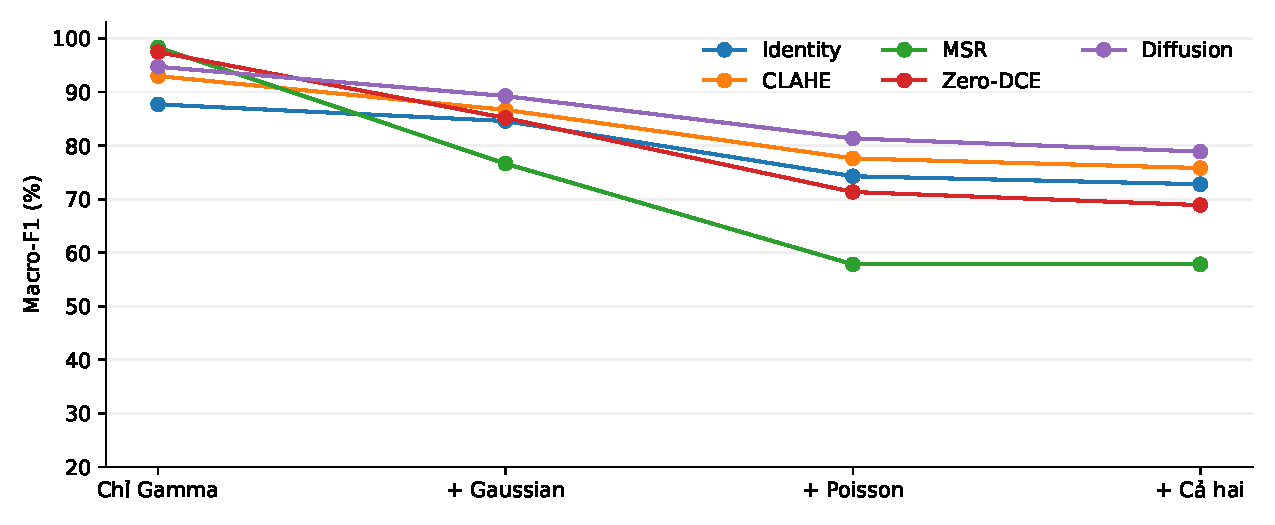
\includegraphics[width=.86\linewidth,height=5cm,keepaspectratio]{ablation.pdf}
\captionnote{430 ảnh, 288 lượt; giữ $\gamma_d=2,2$, checkpoint và tham số enhancer. Hai loại nhiễu chưa cân bằng năng lượng.}

\end{frame}

\paperreference{}
\begin{frame}{5.7. Thứ tự không có quy tắc tốt nhất cho mọi bộ lọc}

\textbf{Cặp Gaussian--CLAHE, full-test}\par
Giữ cùng kernel, sigma, clip limit và tile grid.\par\vspace{3mm}
CLAHE rồi Gaussian trừ Gaussian rồi CLAHE:\par
$\Delta$ Macro-F1 trung bình: $+0,17$ / $+0,11$ / $+0,15$ điểm phần trăm.\par\vspace{3mm}
Một số checkpoint/noise seed có chiều ngược lại.\par
Gaussian--Gamma chỉ so cả hai thứ tự trên validation và subset.
\takeaway{Khoảng cách nhỏ chưa chứng minh ưu thế thống kê.}

\end{frame}

\paperreference{}
\begin{frame}{5.8. Phân tích cả mẫu được giúp và bị làm sai}

\textbf{Gaussian rồi Gamma, mức vừa, full-test}\par\vspace{3mm}
Sửa đúng trung bình: \alert{1.472,67 ảnh/lượt}.\par
Làm sai trung bình: \alert{29,22 ảnh/lượt}.\par
Tăng ròng: 1.443,44 ảnh, tương ứng 11,43 điểm phần trăm Accuracy.\par\vspace{4mm}
$\Delta\mathrm{Accuracy}=100(H-D)/12.630$.\par
Không dùng $H-D$ thay cho chênh lệch Macro-F1.
\captionnote{Trung bình qua noise seed và checkpoint; không coi các seed là ảnh nguồn độc lập.}

\end{frame}

\paperreference{}
\begin{frame}{5.9. Macro-F1 tốt hơn vẫn còn lớp khó}

\centering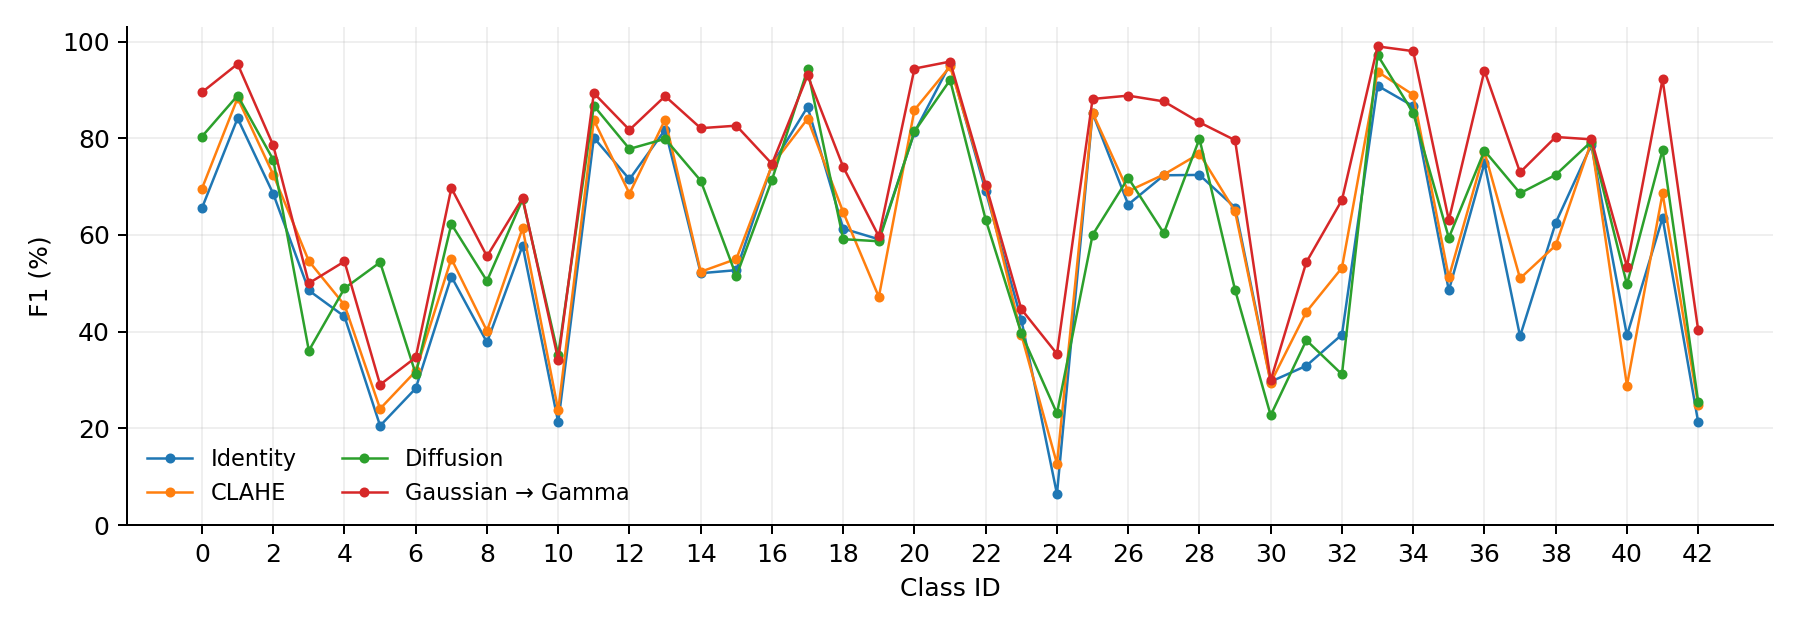
\includegraphics[width=.95\linewidth,height=5cm,keepaspectratio]{per_class_severe.png}
\captionnote{F1 từng lớp full-test mức nặng. Dự đoán và ma trận được kiểm chứng; dữ liệu vẫn là suy giảm mô phỏng.}

\end{frame}

\paperreference{}
\begin{frame}{6.1. Quy trình tiền xử lý được chọn}

\begin{enumerate}
\item Crop ROI + lề 5\%, RGB $64\times64$, chia 255.
\item Gaussian $5\times5$, $\sigma=0,8$, biên phản xạ.
\item Gamma $\alpha=0,8$ trên float32, không lượng tử hóa 8 bit.
\item Resize $224\times224$, normalize ImageNet một lần.
\item Cùng ResNet-18 cố định, 43 lớp.
\end{enumerate}
\takeaway{Ảnh thiếu sáng thực đi trực tiếp vào xử lý, không làm tối thêm.}
\captionnote{Độ trễ khối Gaussian--Gamma khoảng 0,293 ms/ảnh; chưa phải tốc độ toàn hệ thống. Đối chứng dùng lại từ phiên khác.}

\end{frame}

\paperreference{}
\begin{frame}{6.2. Kết luận và giới hạn}

\textbf{Ba kết luận}\par
Khử nhiễu kết hợp tăng sáng cải thiện F1 trong giao thức đã xét.\par
PSNR/SSIM không bảo đảm giữ đặc trưng phân lớp.\par
Thứ tự phụ thuộc phép xử lý và cấu hình.\par\vspace{3mm}
\textbf{Giới hạn}\par
ROI có sẵn, nhiễu RGB tổng hợp, một kiến trúc CNN.\par
Chưa đánh giá camera đêm thực, detector hoặc video.\par
Chưa kết luận ý nghĩa thống kê cho các khoảng cách nhỏ.
\par\vspace{3mm}{\color{Teal}\large\bfseries Cảm ơn thầy cô và các bạn!}

\end{frame}

\end{document}
